\section{System Architecture}
\label{sec:architecture}

In this section, we briefly outline an architecture for providing
consistency prediction, monitoring and verification given our experiences
implementing them for two production NoSQL stores---Cassandra and
Voldemort. The techniques used to implement PBS are applicable to any
system for which we can model the replication protocol used and only
require lightweight profiling in the data store.
%require only lightweight latency profiling in the underlying data
%store.

%Introductory paragraph explaining the system architecture. Explain that our
%approach is to make PBS a shim layer on top of existing server code. Latency
%measurements etc.

\begin{figure}
\centering
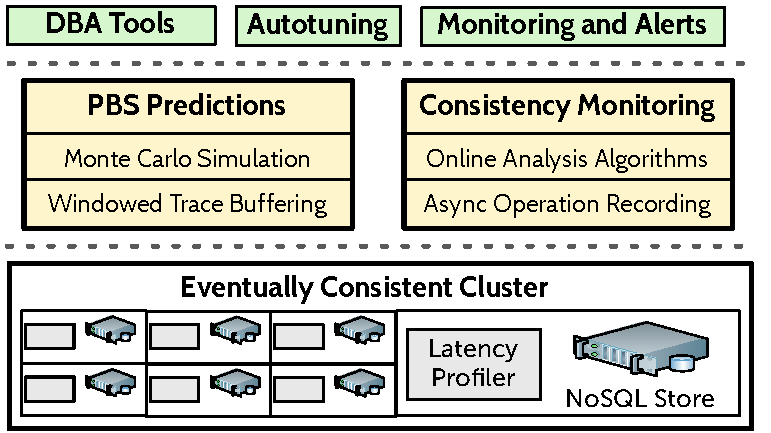
\includegraphics[width=\columnwidth]{figs/cluster-arch.pdf}
\caption{Diagram showing how PBS metrics can be integrated into an
  existing NoSQL datastore. The PBS prediction module and consistency
  monitoring module provide the metrics used by higher level applications like
  dynamic query tuning, monitoring, and diagnostic tools.}
\label{fig:pbs-sys-arch}
\end{figure}


\subsection{Database Architecture}
\label{sec:dbarch}

The lower two layers in Figure~\ref{fig:pbs-sys-arch} show the changes
that are required to integrate PBS-style metrics into an existing
distributed database. In each replica, or storage node, we perform
lightweight latency profiling by piggybacking timestamps on messages
exchanged between servers. This data is subsequently processed by two
separate modules that provide consistency prediction and monitoring.
These modules are cleanly separable from the main data
store implementation and can be easily adapted to different systems.\\
%Walk through the system diagram - Explain what each component does. In
%particular explain how the latency collector feeds into the PBS prediciton
%module and how the Monte-Carlo simulation can be run using this data.
\textbf{PBS Prediction:} The PBS prediction module is responsible for
calculating the $t$-visibility and $k$-staleness of the
datastore. This module records the latencies for relevant operations
in the data store (in Dynamo-style systems, the respective latencies
for writes, acks, reads, and responses---the PBS \textit{WARS} model)
that are sent during replication.  The prediction module tracks a
moving window of recent latencies across servers, and, when an
end-user (or higher-level component) requests a consistency
prediction, the module uses the latencies to provide a
prediction. Predictions are performed using Monte Carlo analysis, and
the module simulates the interactions between thousands of read and
write requests %in the underlying replication mechanism 
that each behave stochastically according to the observed distributions. This
allows us to estimate $t$-visibility, $k$-staleness, and latency for
the operations under a range of parameter choices: replication
factors, anti-entropy rates, and node failures. In our Cassandra
implementation, we found that the prediction typically finishes within
a second for thousands of trials.

%Talk about how the simulation can be triggered by either the database
%administration tool or the Consistency SLA verifier module. The consistency sla
%verifier accepts SLA specifications from clients and periodically triggers the
%prediction module - This module also completes the loop and adjusts the value of
%N,R and W until the consistency SLA is met.
\noindent{\textbf{Consistency Monitoring:}} While predictions are useful, it is
also beneficial to know what consistency a data store is actually providing.
While PBS gives a probability distribution function (PDF) of reads that are
consistent after a fixed amount of time, consistency monitoring amounts to
integrating over the PDF: what percent of reads are actually consistent?
Black-box monitoring is somewhat more difficult than predictions because
determining the latest write effectively requires consensus about the value of
the latest write. This requires substantially more coordination than prediction
but is the subject of considerable ongoing research~\cite{hotdep}. 

On the other hand, our verifier for Cassandra uses white-box techniques similar
to the PBS predictor. Even though an operation might complete with a reply
from a single replica (say $R$=$1$), the monitoring module asynchronously collects 
data from other replicas as well. In addition to this, the monitoring modules
periodically exchange timing metadata for writes and this is passed to an online
analysis algorithm that detects potential violations of consistency.

\subsection{Userspace tools}


As we described in Section~\ref{sec:dynamic}, one of the use cases of
consistency prediction is that we can build tools that use metrics to
provide SLAs on consistency. This can be accomplished by a standalone
module that tracks the consistency and latency profile of queries over
time. Database administrators can specify the SLA required in terms of
maximum acceptible values for (a combination of) $t$-visibility,
$k$-staleness, and operation latency. The auto-tuning module
periodically triggers the PBS predictor. Based on the predictions,
replication parameters are adjusted to ensure that the SLA is met
while minimizing the latency observed. The number of possible states
is limited for small values of $N$, so our current implementation
performs a complete search over the state space.

%Finally talk about how the database administration tool can also trigger the pbs
%prediction. Explain how this works with respect to nodetool and the flexibility
%they have with respect to the query inteface.
The PBS predictions are not only meant to be used by automated tools
like the auto-tuning module but can also be used by database administrators
to get more insights into the latency-consistency trade-offs for their
deployment. In our Cassandra implementation, we have added a new
command \texttt{predictconsistency} to \texttt{nodetool}, a widely
used administration interface.  The \texttt{predictconsistency}
command provides a flexible interface for performing PBS
prediction. Database administrators can specify the replication factor
($N$, $R$, $W$) to be used and the time at which a read is performed
after a write request. This allows administrators to perform ``what-if''
analysis and project the impact on latency and consistency as their
workload changes.  Finally, we also export the consistency metrics
over a Java MBean interface, meaning any tool that can handle MBean
output can be used to display this data.

%Last talk a little bit about the monitoring tools and how one can export the PBS
%metrics in a time series format and alert the users if some trigger has not been
%meet for the given time period.

Finally, PBS can be used by administrators to monitor the consistency their
datastore is providing them. In contrast to offline consistency
verification schemes~\cite{podc-hpl}, PBS predictions provide a
lightweight mechanism that can be used for monitoring. A monitoring
tool like Ganglia~\cite{massie2004ganglia} or DataStax's
OpsCenter~\cite{datastax-opscenter} can be used to issue periodic PBS
prediction requests and plot the values of $t$-visibility and
$k$-staleness as a timeseries. This can then be integrated with
rule-based alerting systems to page an operator if the value of
$t$-visibility is beyond a particular threshold.
%for an extended time period.
